\documentclass[12pt]{article}

\usepackage[utf8]{inputenc}
\usepackage[greek, english]{babel}
\usepackage{alphabeta}
\usepackage{libertine}
\usepackage{graphicx}
\usepackage{amsmath}

\title{Algorithms \\ Programming exercise 3}
\author{Κωνσταντίνος Νικολούτσος \\ p3170122}
\date{}



\begin{document}

\maketitle


\section{Ασκηση 3.2}
Πατατηρήθηκε οτι υπάρχει τεράστια διαφορά αν χρησιμοποιήσουμε dynamic programming ή greedy. 
Φυσικα βέβαια θα πρέπει να γνωρίζουμε οτι το bruteforce παντα θα μας δίνει την καλύτερη λύση ενω το greedy μπορει να μας δώσει καποια ικανοποιητική λυση. Με λιγα λόγια πληρώνουμε περισσότερο χρόνο (πολυπλοκότητα) για να πάρουμε τα καλυτερα αποτελέσματα.

\subsection{Πολυπλοκότητες}
\begin{itemize}
	\item BruteForce εχει: $O(2^n*n^2)$ , n είναι ο αριθμός των κόμβων του δικτύου
	\item Greedy έχει: $Ο(n^3)$, n είναι ο αριθμός των κόμβων του δικτύου
\end{itemize}

\begin{center}
	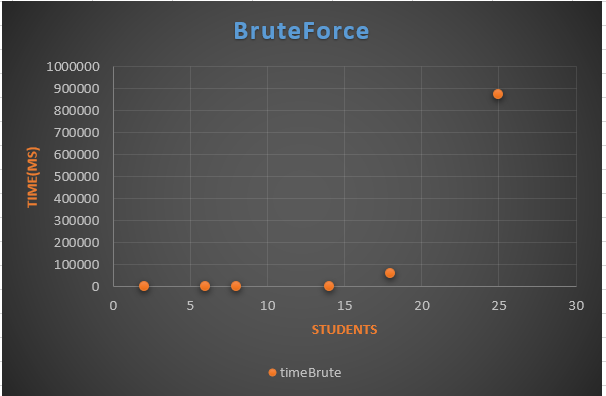
\includegraphics[scale = 0.6]{graph_brute.png}
\end{center}

\begin{center}
	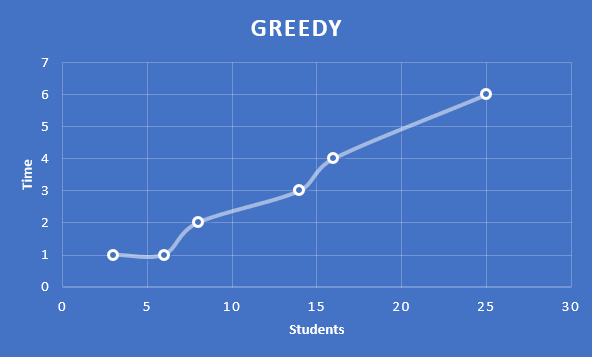
\includegraphics[scale = 0.6]{greedy.png}
\end{center}




Η γνώμη μου είναι οτι εξαρτάται απο το πρόβλημα εαν πρέπει να περιμένουμε περισσότερο. 
Πιο αναλυτικά, υπάρχουν προβλήματα για τα οποία ειτε περιμένουμε παραπάνω είτε όχι δεν πρόκειτε να πάρουμε καλύτερη λύση (δηλαδή αν ο greedy δίνει βέλστιστη λύση).


\subsection{Ποιότητα διαφοράς αποτελεσμάτων}
Ο greedy αλγόριμος δεν ειναι σίγουρο οτι θα μας δώσει πάντα την καλύτερη απάντηση. Σε αντίθεση, ο bruteforce αν και κανει αρκετο χρόνο, μας δίνει πάντα την optimum λύση!
Για παράδειγμα στην παρακάτω εικόνα βλέπουμε οτι ο bruteforce(αριστερα) δίνει την σωστη λύση (πρασινα τικ) ενω ο greedy(δεξιά) δίνει λάθος (κόκκινα χ). Μάλλον οποιος βίαζεται σκοντάφτει!

 \begin{center}
	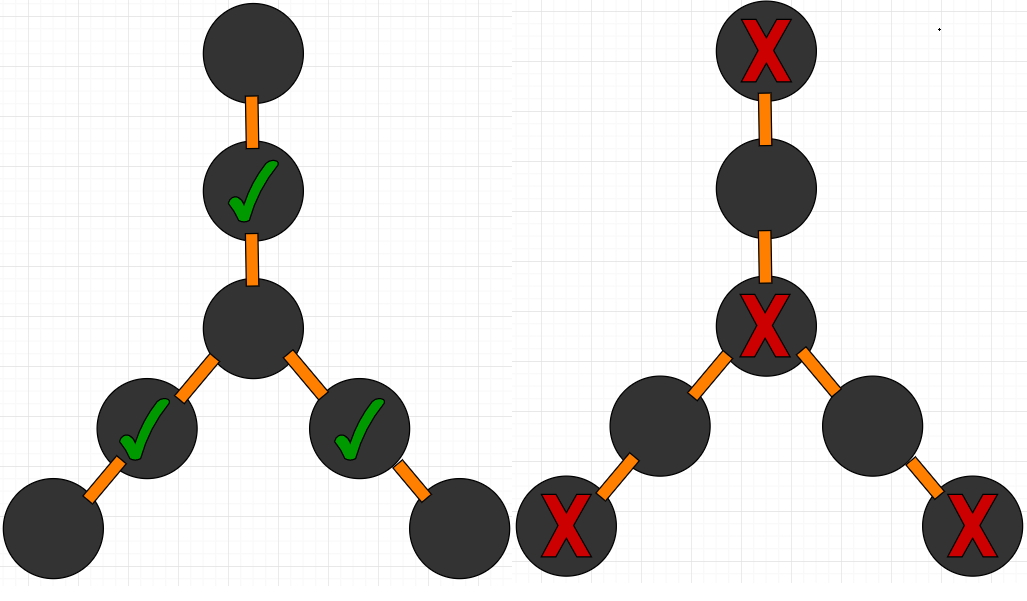
\includegraphics[scale = 0.4]{example.png}
 \end{center}


\newpage
\section{Άσκηση 3.4}

Για να αποδείξουμε οτι το Dominating-set ειναι np-complete προσπαθήσουμε να κάνουμε linear transformation απο κάποιο non deterministic polynomial προβλημα σε αυτο και μετα να παρουμε λύση. $VertexCover\le_P DominatingSet$ \\

Έχοντας ενα Instance (G, k) του Vertex cover θα φτιάξουμε ενα Instance του Dominations set (H, k), όπου το H το φτιάχνουμε παίρνοντας τον G και για καθε ακμή (u,v) προσθέτουμε μια επιπλέον κόμβο και τον συνδέουμε με u,v

Πρώτα παρατηρούμε οτι ο Vertex cover του G ειναι ενα Dominating Set του H.
(Οι καινούργιοι κόμβοι που προσθέσαμε καλύπτονται οποτε ισχυει οτι ειναι dominating set).
Οπότε εαν το G είχε καποιο μικρότερο vertex cover τότε το H θα είχε μικρότερο πλήθος λύσης απο το k.

Παρατηρούμε οτι εαν κόμβος είναι στο D, μπορούμε να τον αντικαταστίσουμε με εναν απο τους δύο γείτονες του και να πάρουμε ενα dominating set. Αξίζει να σημειωθεί οτι οι μόνοι γείτονες του είναι οι δύο αρχικοί κόμβοι και ειναι συνδεμένη μεταξυ τους.

Οπότε μπορουμε να υποθέσουμε οτι ο D περιέχει μόνο τους κόμβους του G. Τώρα, για κάθε ακμή (u,v) στον G ο νέος κομβος ειναι καλυμένος (dominated) απο τον D, οπότε είτε το u ή το v ειναι στο D. Αλλα φυσικά αυτο σημάινει οτι ο D ειναι ενα vertex cover του G.

Kαι αποδείξαμε οτι υπάρχει σχέση μεταξύ vertex cover και dominating set. Αρα δεν γίνεται το dominating σετ να ειναι πιο δύσκολο απο το vertex cover.


 












\end{document} 
